\documentclass[10pt]{amsart}
\usepackage{amsmath,amssymb,amsthm,amsfonts,amscd,flafter,epsf,bm}
\usepackage{color}
\usepackage{tikz}
\usetikzlibrary{patterns}

\begin{document}

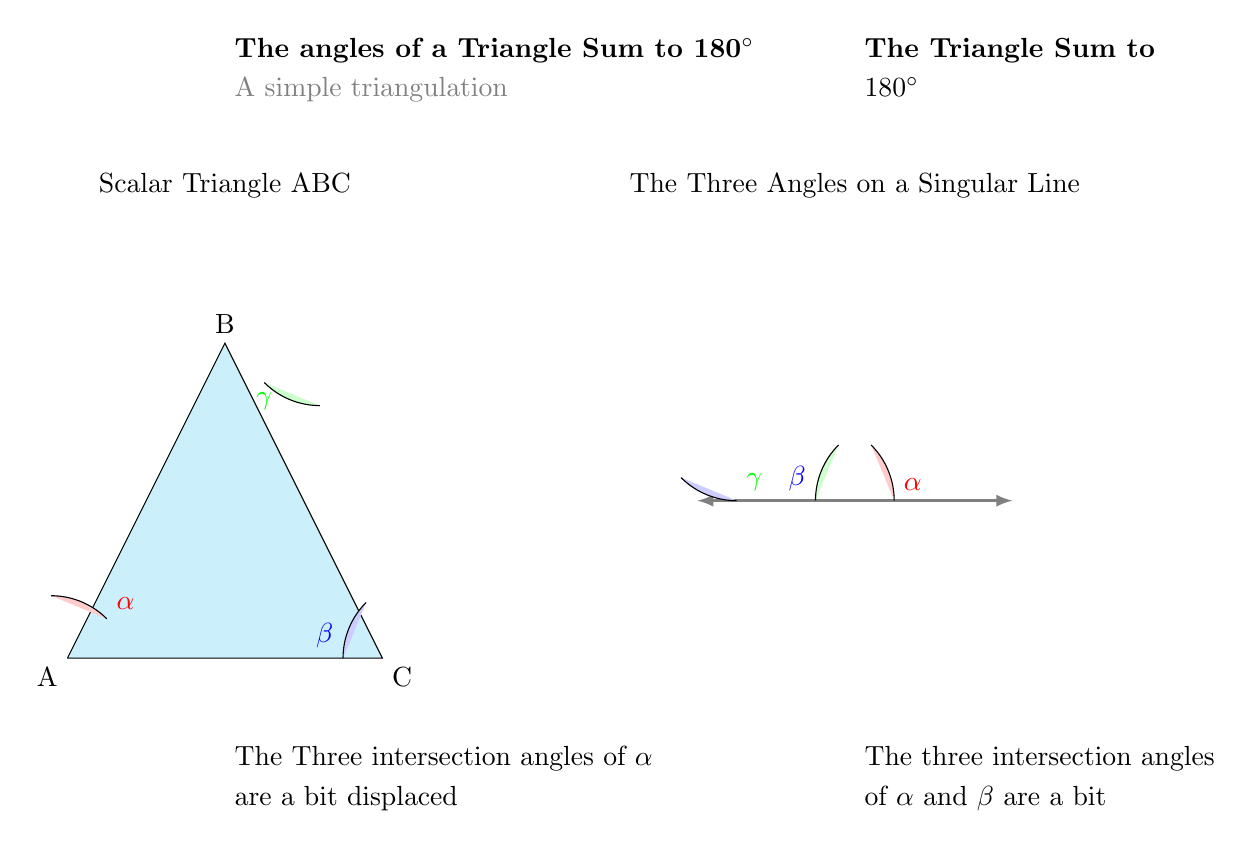
\begin{tikzpicture}


\draw [fill=cyan!20!white] (0,0) -- (4,0) -- (2,4) -- (0,0);
\draw [fill=red!20!white] (0.5,0.5) arc (45:90:1cm);
\draw [fill=green!20!white] (2.5,3.5) arc (225:270:1cm);
\draw [fill=blue!20!white] (3.5,0) arc (180:135:1cm);


\draw (0,0) node[below left] {A};
\draw (2,4) node[above] {B};
\draw (4,0) node[below right] {C};

\draw (0.5,0.5) node[above right] {\textcolor{red}{$\alpha$}};
\draw (2.5,3.5) node[below] {\textcolor{green}{$\gamma$}};
\draw (3.5,0) node[above left] {\textcolor{blue}{$\beta$}};

\draw (2,6) node {Scalar Triangle ABC};

\draw[<->,>=latex,gray,line width=1pt] (8,2) -- (12,2);

\draw [fill=red!20!white] (10.5,2) arc (0:45:1cm);
\draw [fill=green!20!white] (9.5,2) arc (180:135:1cm);
\draw [fill=blue!20!white] (8.5,2) arc (270:225:1cm);

\draw (10.5,2) node[above right] {\textcolor{red}{$\alpha$}};
\draw (9.5,2) node[above left] {\textcolor{blue}{$\beta$}};
\draw (8.5,2) node[above right] {\textcolor{green}{$\gamma$}};

\draw (10,6) node {The Three Angles on a Singular Line};

\draw (2,-1) node[below right] {The Three intersection angles of $\alpha$};
\draw (2,-1.5) node[below right] {are a bit displaced};
\draw (10,-1) node[below right] {The three intersection angles};
\draw (10,-1.5) node[below right] {of $\alpha$ and $\beta$ are a bit};
\draw (2,8) node[below right] {\textbf{The angles of a Triangle Sum to 180$^\circ$}};
\draw (2,7.5) node[below right] {\textcolor{gray}{A simple triangulation}};
\draw (10,8) node[below right] {\textbf{The Triangle Sum to}};
\draw (10,7.5) node[below right] {180$^\circ$};

\end{tikzpicture}

\end{document}